% ============================================================
%  Test problems.  Input this AFTER numerical_setup.tex and planar_solver.tex.
% ============================================================
\section{Test problems}
\label{sec:tests}

Three problems are used. Two are one-dimensional Riemann problems chosen so
that the slow magnetosonic waves carry a visible part of the structure: they
are the problems on which an exact Riemann solver should be seen to do
something an approximate one cannot, since HLLD carries no slow wave at all.
Both are non-coplanar, so the seven-wave solver is well posed on them, and
both are solved by the warm-start network of Sect.~\ref{sec:setup:exact} from
its own seed without a retry, so the whole pipeline is exercised on cases
whose answer is known. The third is the two-dimensional magnetic rotor, on
which the scheme is actually run.

\subsection{One-dimensional problems where the slow waves matter}
\label{sec:tests:1d}

A shock tube is a single Riemann problem read along the rays
$\xi = (x - x_0)/t$, so its exact solution at the output time is available at
every cell from the same solver, with no resolution study and no
discretisation error of its own. The comparisons below are therefore
measured against the truth rather than against a finer grid. Each problem is
run on 400 cells to $t = 0.4$ with the interface at $x_0 = 0.5$, the PLM/MC
reconstruction of Sect.~\ref{sec:setup:evolution}, and either the HLLD flux
or the exact flux with HLLD as its fallback. On a shock tube the weak-jump
gate of Sect.~\ref{sec:setup:exact} hands most interfaces to HLLD, because
the two reconstructed states are identical across all of them but the few
that sit inside a fan; measured over the runs below the exact solver supplies
the flux on $26.7\%$ to $45.4\%$ of faces, a fraction that grows through the
run as the fans widen. Both arms are otherwise identical, so the comparison
isolates the flux.

\subsubsection{Balsara test 5}
\label{sec:tests:balsara5}

The first problem is test 5 of Balsara (2001), reproduced in Table~4 of
Giacomazzo \& Rezzolla (2006): the generic case in that suite, in which every
primitive variable differs across the interface and all seven waves appear
with comparable strength. In $(\rho, p, v_x, v_y, v_z, B_x, B_y, B_z)$ the
left state is $(1.08, 0.95, 0.40, 0.3, 0.2, 2, 0.3, 0.3)$ and the right
state $(1.00, 1.00, -0.45, -0.2, 0.2, 2, -0.7, 0.5)$, with $\Gamma = 5/3$.
The tangential fields are far from parallel, $\chi = 0.986$ in the measure
of Eq.~(\ref{eq:coplanarity}), against a median of $7.6 \times 10^{-11}$ on
the rotor and $0.65$ in the network's training set, so the problem sits in
the network's home distribution. Both production checkpoints converge the
seven-wave Newton from the bare seed, with no jitter and no retry: the seed
misses the root by $0.03$ in $\ln p_{LF}$ and $\ln|B_{t,CD}|$ and by
$0.06$~rad in $\phi_L$---a seed error of $0.10$ per unknown is where the
Newton's measured convergence begins to fall off---and the two checkpoints
land on the same root.

The solution carries a large rotational discontinuity on the left,
$\phi_L = 1.59$~rad, and its left slow wave sits only $0.0016$ in $\xi$ from
the left Alfv\'en wave---under one cell at this resolution, effectively
degenerate---while on the right the slow wave is well separated from its
Alfv\'en wave ($\xi = 0.364$ against $0.410$, seven cells at $t = 0.4$).
The right side is therefore where the missing wave shows: between the
contact and the right Alfv\'en wave the exact solution has two states,
separated by the slow wave, and HLLD's model has one.

\begin{figure}
\centering
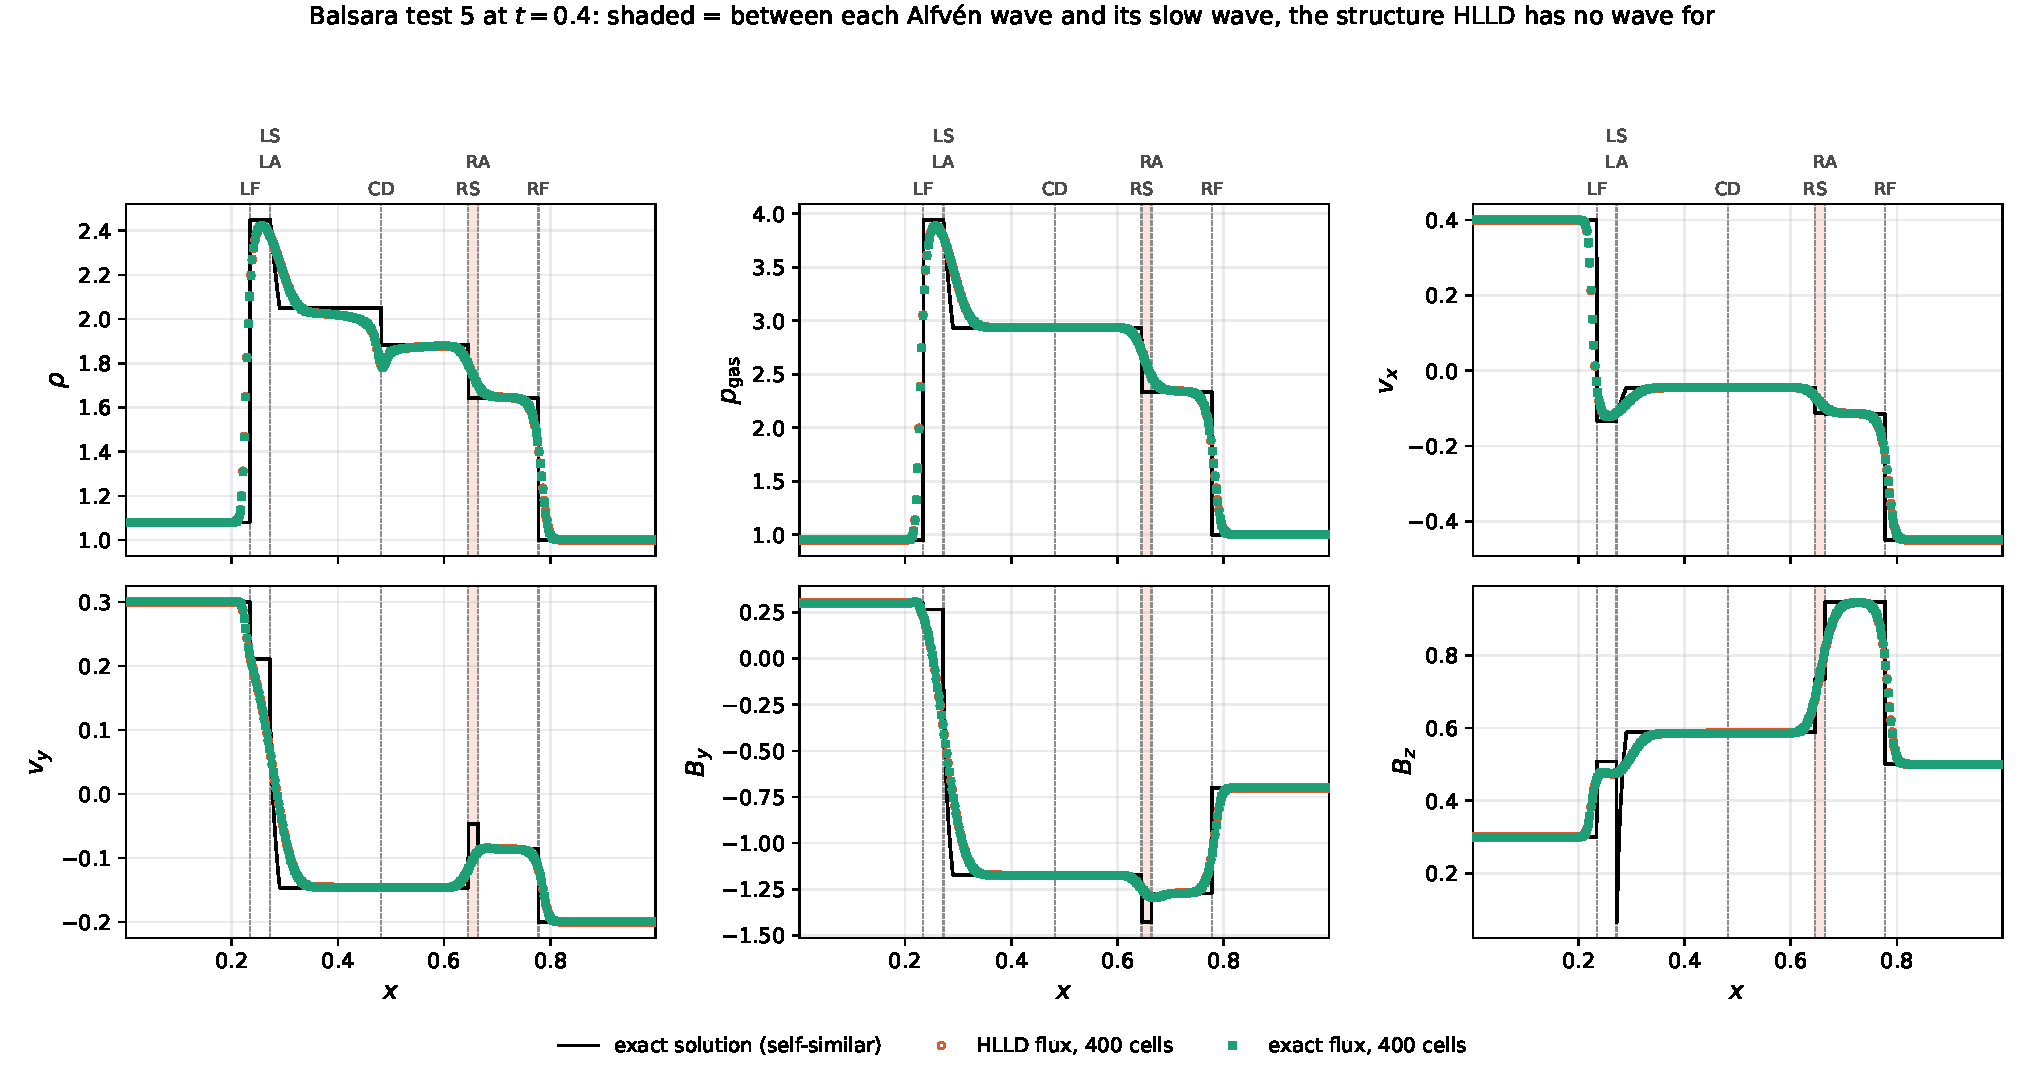
\includegraphics[width=\textwidth]{figs/balsara5_slowwave.pdf}
\caption{Balsara test 5 at $t = 0.4$ on 400 cells. Black is the exact
self-similar solution, orange the HLLD flux, green the exact flux. The
shaded bands lie between each Alfv\'en wave and its slow wave. The two
numerical solutions are indistinguishable at this scale: the orange symbols
are hidden behind the green almost everywhere.}
\label{fig:balsara5}
\end{figure}

Figure~\ref{fig:balsara5} shows the result. The exact flux was used on
$45.4\%$ of faces and cost $19\,482$~s against $62$~s for HLLD, a factor of
$314$. In $L_1$ against the exact solution it is better on every variable,
uniformly by about one per cent:

\begin{center}
\begin{tabular}{lccc}
\toprule
 & HLLD & exact & ratio \\
\midrule
$\rho$ & $3.962\times10^{-2}$ & $3.910\times10^{-2}$ & $0.987$ \\
$p$    & $6.627\times10^{-2}$ & $6.549\times10^{-2}$ & $0.988$ \\
$v_x$  & $1.139\times10^{-2}$ & $1.124\times10^{-2}$ & $0.987$ \\
$B_y$  & $3.516\times10^{-2}$ & $3.494\times10^{-2}$ & $0.994$ \\
$B_z$  & $1.622\times10^{-2}$ & $1.604\times10^{-2}$ & $0.989$ \\
\bottomrule
\end{tabular}
\end{center}

A one per cent gain for a factor of $314$ in cost. Note also that this
problem's \emph{left} slow wave is degenerate at this resolution --- it sits
$0.3$ cells from its Alfv\'en wave --- so the only resolved slow-wave
structure is the right-hand band, $7.4$ cells wide, and both schemes
reproduce it identically.

\subsubsection{A constructed slow-shock tube}
\label{sec:tests:slowshock}

The second problem is built rather than chosen. Picking two states and
hoping the waves that appear are the ones wanted is how test problems are
usually made; instead we construct the solution with the exact solver's own
wave routines and read the right state off the end of it, so that the slow
shock has exactly the strength asked for and the whole solution is known by
construction. Starting from a left state at plasma $\beta = 0.04$ inside the
rotor envelope, $(\rho, p, v_x, v_y, v_z, B_x, B_y, B_z) =
(1, 0.1, 0.1, 0, 0, 1, 2, 0)$, we cross a weak fast wave
($P_{\rm tot} \times 1.15$), a rotational discontinuity of $0.5$~rad, and a
slow shock that halves $|B_t|$, then double the density across a contact.
The right-going family is silent. The right state that results is
$(8.0531, 2.3147, -0.2777, -0.7330, 0.0518, 1, 0.8368, 0.5475)$, given to
full precision in \texttt{configs/slow\_shock\_tube.yaml}, which
\texttt{scripts/make\_slow\_shock\_tube.py} regenerates from those four
choices.

The low $\beta$ is what makes the slow shock large: it has magnetic energy
to convert. Across it the density rises by $3.74$ (the strong-shock limit
for $\Gamma = 5/3$ is $4$), the gas pressure by $20.5$, from $0.113$ to
$2.32$, and the transverse velocity is deflected from $v_y = -0.07$ to
$-0.73$, while $|B_t|$ falls from $2.40$ to $1.00$. Almost all of the
structure in this problem is in the one wave HLLD does not have. A further
$|B_t|$ drop changes little (a factor of $8$ reaches $4.09$ and $24.9$): the
shock is near its strong limit already.

One detail of the construction is worth recording, because it cost an
afternoon and says something about the seven-wave unknowns. A relativistic
slow shock does not deliver the field direction it is aimed at: with
transverse velocity the downstream $B_t$ is twisted in the lab frame, here
by $4.55^\circ$, so the naive assignment $\psi_{CD} = \psi_L + \phi_L$
leaves the slow wave's slack component (Sect.~\ref{sec:setup:exact}) at
$1.6 \times 10^{-2}$ even though all four contact jumps vanish. The
consistent $\psi_{CD}$ is the fixed point of the delivered angle, found by
a secant iteration on that slack (four steps to $10^{-15}$; a plain
fixed-point update diverges). With it the constructed unknowns satisfy the
full residual to $5.8 \times 10^{-15}$. The problem is non-coplanar,
$\chi = 0.547$, and both production checkpoints converge from the bare seed
to the constructed root within $6 \times 10^{-10}$, from seed errors of
$0.05$--$0.14$ in the log-magnitudes and up to $0.2$~rad in the angles.

At $t = 0.4$ the left slow shock stands at $x = 0.364$, $0.006$ (two and a
half cells) to the right of the Alfv\'en wave at $0.358$, and the contact at
$0.389$; the ten cells between the slow shock and the contact hold the
post-shock state.

\begin{figure}
\centering
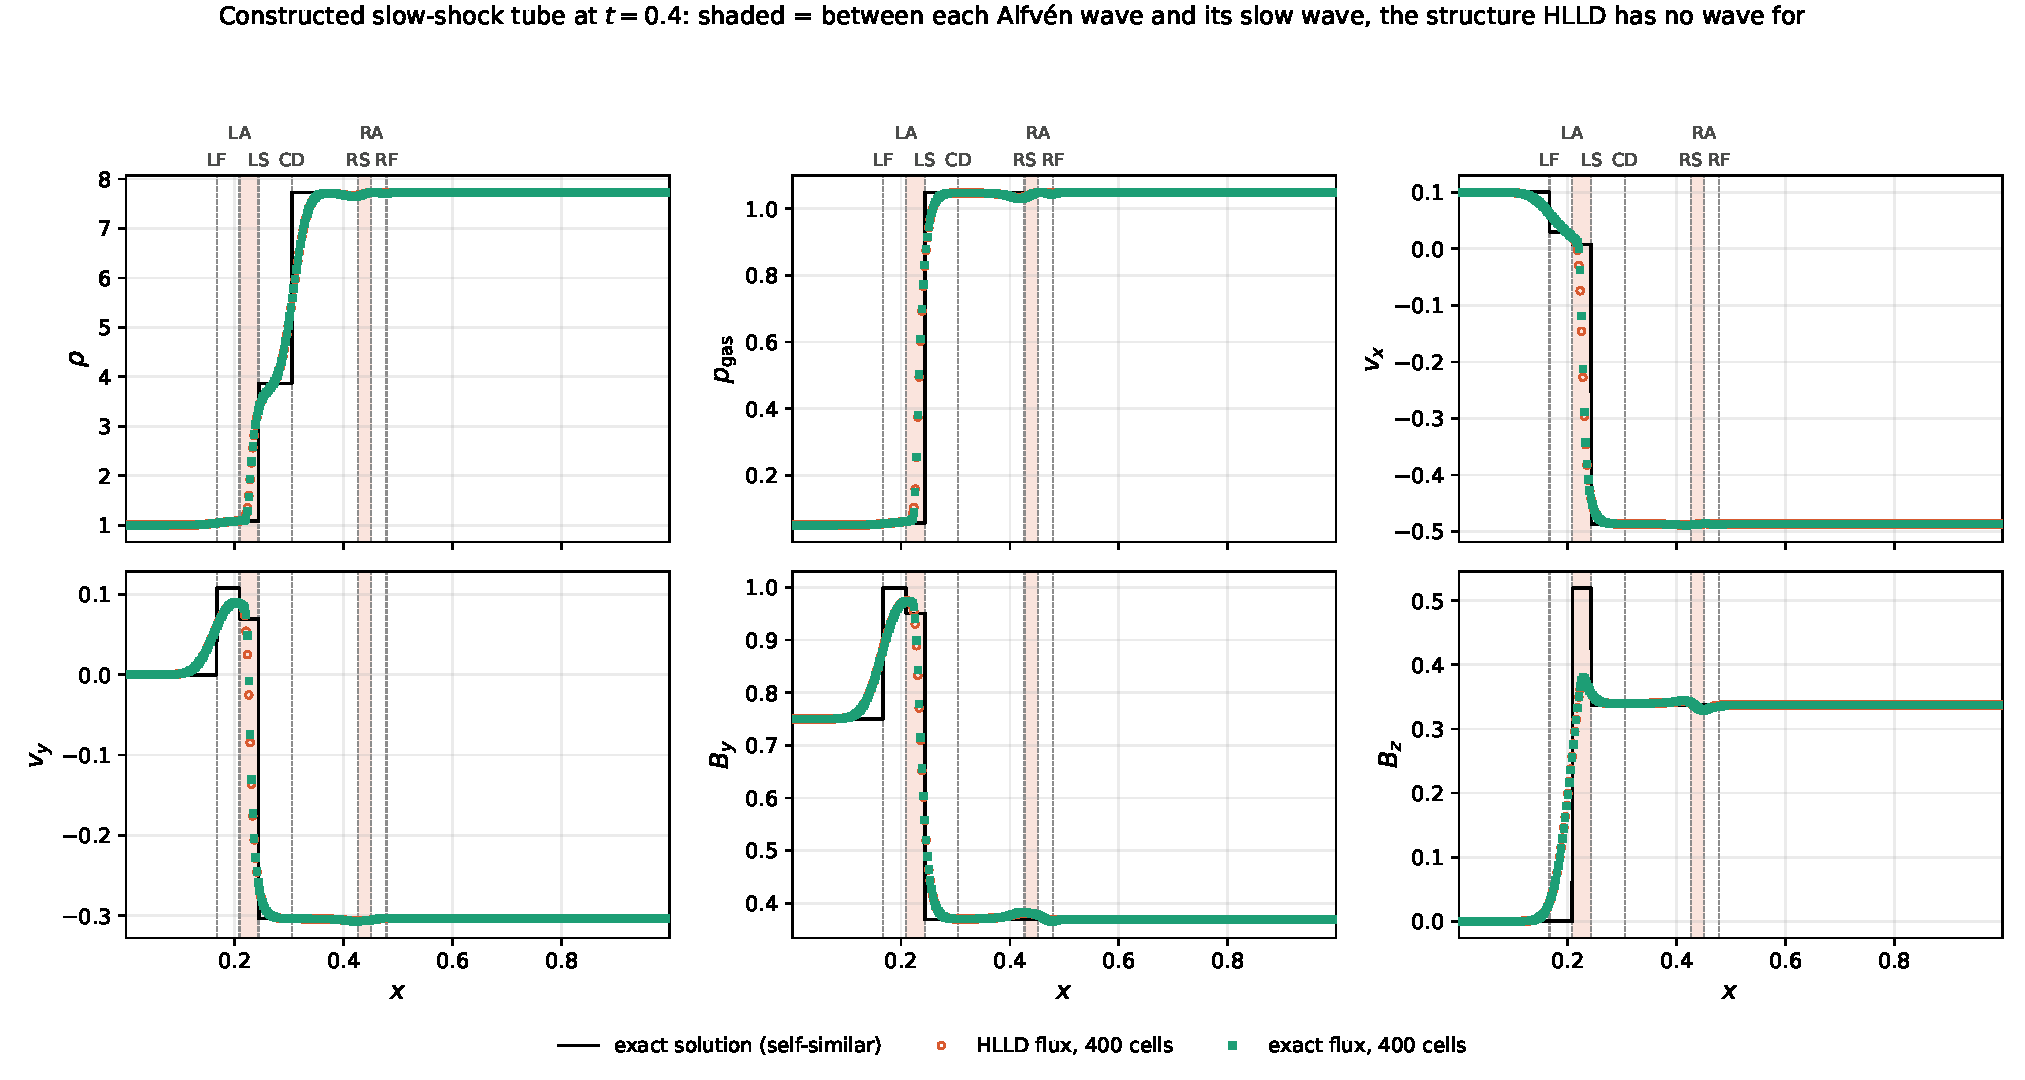
\includegraphics[width=\textwidth]{figs/slow_shock_tube.pdf}
\caption{The constructed slow-shock tube at $t = 0.4$ on 400 cells, drawn as
in Fig.~\ref{fig:balsara5}. Here both slow-wave bands are resolved, $13.9$
cells on the left and $9.8$ on the right, and both schemes reproduce the
post-shock state; the exact flux has no advantage.}
\label{fig:slowshock}
\end{figure}

The exact flux was used on $26.7\%$ of faces and cost $7220$~s against
$81$~s for HLLD, a factor of $90$. It is \emph{not} better. In $L_1$ it wins
on the velocities by $1$--$3\%$, ties on the fields to three digits, and
\emph{loses} on density ($1.006$) and pressure ($1.014$). On the problem
built to give an exact Riemann solver its best case, the flux buys nothing.

The reason is visible in the figure and is worth stating carefully. Both
schemes resolve the intermediate state between the Alfv\'en wave and the
slow shock, both overshoot its plateau by the same amount, and both relax to
the same post-shock values. HLLD carries no slow wave, yet it reproduces the
slow-shock state correctly, because the state behind a shock is fixed by the
jump conditions and those are enforced by conservation whatever waves the
flux function models. What the flux controls is the dissipation inside the
transition, and there the error is set by the PLM/MC reconstruction across a
structure with three discontinuities packed into fourteen cells, not by
which Riemann problem the face solved.

An earlier version of this problem makes the point sharper. Built with
$B_n = 1$ and $|B_t| = 2$, it had a \emph{stronger} slow shock
($\rho \times 3.74$, $p \times 20.5$) but its Alfv\'en-to-slow band was only
$2.5$ cells wide. There the exact flux did win, by $2$--$4\%$ on every
variable. The gain came from a zone that neither scheme resolves, where the
two fluxes differ because both are wrong, and it evaporated as soon as the
same structure was made resolvable. Ordering the three problems by how well
the slow-wave structure is resolved --- $2.5$ cells, $7.4$ cells, $13.9$
cells --- the advantage of the exact flux falls monotonically from $2$--$4\%$
through $1\%$ to nothing. That is the opposite of the expected trend, and it
is the one-dimensional counterpart of the two-dimensional measurement of
Sect.~\ref{sec:tests:rotor}, reached by an independent route.

\paragraph{How much of the solver is actually used.} These runs are hybrids,
and the fallback is worth reporting rather than hiding behind the coverage
figure. Instrumenting both problems at $t \approx 0.12$ and averaging over
twenty consecutive sweeps of $401$ interfaces:

\begin{center}
\begin{tabular}{lcc}
\toprule
per sweep, of 401 interfaces & slow-shock tube & Balsara 5 \\
\midrule
weak-jump gate $\rightarrow$ HLLD & $333.1$ ($83.1\%$) & $300.1$ ($74.8\%$) \\
attempted                          & $67.9$ ($16.9\%$)  & $100.9$ ($25.2\%$) \\
\quad of which exact               & $36.4$             & $57.7$ \\
\quad of which fell back           & $31.5$             & $43.2$ \\
\midrule
\textbf{fallback rate on attempted} & $\mathbf{46.4\%}$ & $\mathbf{42.8\%}$ \\
\bottomrule
\end{tabular}
\end{center}

So roughly two attempted faces in five are lost on both problems, against
$22\%$ on the rotor --- the rate is a property of these problems, not of one
of them. Of the failures, only $0.9$ and $8.6$ respectively are rejected by
the wave-ordering gate, and none fail verification or the ray read
($n_{\rm verified} = n_{\rm exact}$ exactly on both): essentially all of them
are the seven-wave Newton failing to converge at all. One structural reason is that
the five-wave planar rescue, which covers $93.5\%$ of rotor interfaces,
never fires here --- these problems are deliberately non-coplanar, so the
planar family cannot represent them. The rotor's higher success rate leans
on a rescue path that is unavailable precisely where the seven-wave solver
should be most at home.

\paragraph{One run with nothing gated away.} The figures above are hybrids,
so the obvious objection is that the gate is hiding something --- that the
interfaces handed to HLLD are exactly the ones where an exact flux would
have mattered. We tested this directly by repeating the slow-shock tube at
$200$ cells twice, identical but for the gate: once as usual, and once with
$\tau_{\rm weak} = 0$ and the upwind skip disabled, so that \emph{every}
interface is attempted. Counts are from the final sweep, where the fans are
widest:

\begin{center}
\begin{tabular}{lcc}
\toprule
of 201 interfaces, final sweep & gated & nothing gated \\
\midrule
weak-jump gate $\rightarrow$ HLLD & $100$ & $0$ \\
attempted                          & $101$ ($50.2\%$) & $201$ ($100\%$) \\
exact                              & $58$ ($28.9\%$)  & $157$ ($\mathbf{78.1\%}$) \\
fell back                          & $43$             & $44$ \\
\midrule
fallback rate on attempted         & $42.6\%$ & $\mathbf{21.9\%}$ \\
wall time                          & $1724$~s & $12818$~s \\
\bottomrule
\end{tabular}
\end{center}

Two things follow. First, the fallback rate on attempted interfaces
\emph{halves} when the gate is removed, from $42.6\%$ to $21.9\%$. That is
not an improvement in the solver but a statement about what the gate
removes: the near-uniform interfaces are easy, and gating them away leaves
an attempted set enriched in hard ones. The honest ceiling for this solver
on this problem is therefore the $78.1\%$ of \emph{all} faces reached with
nothing gated --- and, equivalently, the $44$ interfaces per sweep that
resist it are the same $44$ either way.

Second, and more decisively: the two solutions are the same. The largest
relative difference between the gated and the fully exact run over all cells
is $9.5\times10^{-4}$, in $B_z$; in density it is $2.2\times10^{-4}$. In
$L_1$ they agree to four digits on every variable, and both remain slightly
\emph{worse} than HLLD in density and pressure. Paying a further factor of
$7.4$ in cost to raise exact coverage from $28.9\%$ to $78.1\%$ changes the
answer by one part in a thousand. The gate is not concealing a result, and
the flux is not where the error lives.

\subsection{The magnetic rotor}
\label{sec:tests:rotor}
\label{sec:setup:rotor}

The two-dimensional magnetic rotor is used throughout. A dense cylinder of
radius $r_0 = 0.1$ and density $\rho = 10$ rotates rigidly with angular
velocity $\omega = 9.95$, so that its rim moves at $v = 0.995$ and reaches a
Lorentz factor of about ten, inside a static ambient medium of density
$\rho = 1$. Pressure is uniform, $p = 1$, the field is uniform,
$\mathbf{B} = (1, 0, 0)$, and the adiabatic index is $\Gamma = 5/3$. The
cylinder edge is sharp, with no taper, which is the harder and the standard
form of the test. The domain is $[-0.5, 0.5]^2$ with outflow boundaries, and
the solution is evolved to $t = 0.4$.

Because the initial data are invariant under a rotation by $\pi$ about the
axis, the continuum solution satisfies
$\rho(-\mathbf{r}) = \rho(\mathbf{r})$,
$\mathbf{v}(-\mathbf{r}) = -\mathbf{v}(\mathbf{r})$ and
$\mathbf{B}(-\mathbf{r}) = \mathbf{B}(\mathbf{r})$ at all times. We monitor
the violation of this symmetry as a diagnostic. It is reported rather than
bounded: where the exact solver owns some interfaces and not others, the
fallback pattern need not respect the symmetry, so the measured violation is
of the order of the truncation error and is informative rather than a test of
correctness.
